% This is "sig-alternate.tex" V1.9 April 2009
% This file should be compiled with V2.4 of "sig-alternate.cls" April 2009
%
% This example file demonstrates the use of the 'sig-alternate.cls'
% V2.4 LaTeX2e document class file. It is for those submitting
% articles to ACM Conference Proceedings WHO DO NOT WISH TO
% STRICTLY ADHERE TO THE SIGS (PUBS-BOARD-ENDORSED) STYLE.
% The 'sig-alternate.cls' file will produce a similar-looking,
% albeit, 'tighter' paper resulting in, invariably, fewer pages.
%
% ----------------------------------------------------------------------------------------------------------------
% This .tex file (and associated .cls V2.4) produces:
%       1) The Permission Statement
%       2) The Conference (location) Info information
%       3) The Copyright Line with ACM data
%       4) NO page numbers
%
% as against the acm_proc_article-sp.cls file which
% DOES NOT produce 1) thru' 3) above.
%
% Using 'sig-alternate.cls' you have control, however, from within
% the source .tex file, over both the CopyrightYear
% (defaulted to 200X) and the ACM Copyright Data
% (defaulted to X-XXXXX-XX-X/XX/XX).
% e.g.
% \CopyrightYear{2007} will cause 2007 to appear in the copyright line.
% \crdata{0-12345-67-8/90/12} will cause 0-12345-67-8/90/12 to appear in the copyright line.
%
% ---------------------------------------------------------------------------------------------------------------
% This .tex source is an example which *does* use
% the .bib file (from which the .bbl file % is produced).
% REMEMBER HOWEVER: After having produced the .bbl file,
% and prior to final submission, you *NEED* to 'insert'
% your .bbl file into your source .tex file so as to provide
% ONE 'self-contained' source file.
%
% ================= IF YOU HAVE QUESTIONS =======================
% Questions regarding the SIGS styles, SIGS policies and
% procedures, Conferences etc. should be sent to
% Adrienne Griscti (griscti@acm.org)
%
% Technical questions _only_ to
% Gerald Murray (murray@hq.acm.org)
% ===============================================================
%
% For tracking purposes - this is V1.9 - April 2009

\documentclass{sig-alternate}
\usepackage[usenames,dvipsnames]{color}
\usepackage{amsmath,multirow,alltt,listings,clrscode,pifont}
\usepackage{graphicx}
\usepackage{algorithm, url}
\lstloadlanguages{Java,C++}
\lstset{language=Java,frame=single,captionpos=b,basicstyle=\small}
\def\mc#1{\multicolumn{2}{c|}{#1}}
\def\edit#1{{\color{OrangeRed} #1}}
\newcommand{\argmax}{\operatornamewithlimits{argmax}}
\newcommand{\argmin}{\operatornamewithlimits{argmin}}
\newcommand{\method}[1]{{\sc{#1}}}
\newcommand{\daat}{{\method{daat}}}
\def\edit#1{{\color{OrangeRed} #1}}
\def\review#1{{\color{Cerulean} #1}}
\begin{document}
%
% --- Author Metadata here ---
\conferenceinfo{SIGIR}{'13 Dublin, Ireland}
%\CopyrightYear{2007} % Allows default copyright year (20XX) to be over-ridden - IF NEED BE.
%\crdata{0-12345-67-8/90/01}  % Allows default copyright data (0-89791-88-6/97/05) to be over-ridden - IF NEED BE.
% --- End of Author Metadata ---

\title{Improved Dynamic Optimization of Field-Based \\Retrieval Models}
%
% You need the command \numberofauthors to handle the 'placement
% and alignment' of the authors beneath the title.
%
% For aesthetic reasons, we recommend 'three authors at a time'
% i.e. three 'name/affiliation blocks' be placed beneath the title.
%
% NOTE: You are NOT restricted in how many 'rows' of
% "name/affiliations" may appear. We just ask that you restrict
% the number of 'columns' to three.
%
% Because of the available 'opening page real-estate'
% we ask you to refrain from putting more than six authors
% (two rows with three columns) beneath the article title.
% More than six makes the first-page appear very cluttered indeed.
%
% Use the \alignauthor commands to handle the names
% and affiliations for an 'aesthetic maximum' of six authors.
% Add names, affiliations, addresses for
% the seventh etc. author(s) as the argument for the
% \additionalauthors command.
% These 'additional authors' will be output/set for you
% without further effort on your part as the last section in
% the body of your article BEFORE References or any Appendices.

\numberofauthors{1} 
\author{
% You can go ahead and credit any number of authors here,
% e.g. one 'row of three' or two rows (consisting of one row of three
% and a second row of one, two or three).
%
% The command \alignauthor (no curly braces needed) should
% precede each author name, affiliation/snail-mail address and
% e-mail address. Additionally, tag each line of
% affiliation/address with \affaddr, and tag the
% e-mail address with \email.
%
% 1st. author
 \alignauthor Marc-Allen Cartright\\
        \affaddr{CIIR}\\
        \affaddr{Computer Science Department}\\
        \affaddr{University of Massachusetts Amherst}\\
        \email{irmarc@cs.umass.edu}
}

\date{28 January 2013}

\maketitle
\begin{abstract}
We introduce a method for reformulating field-based retrieval models to significantly improve execution efficiency over standard model implementations. 
Field-based models utilize the document structure to improve retrieval results, representing fields or tagged content as micro-documents within the larger document, resulting in significant improvements over models without field awareness. However processing field information separately in these retrieval models often causes a significant increase in computational cost over their field-less counterparts. Additionally, field-based retrieval models in their original formulation often do not easily lend themselves to dynamic pruning via algorithms such as \method{maxscore} and \method{wand}.

To mitigate these problems we introduce the idea of a $\delta$-function --- the reformulation of a given field-based model that defines the scoring function as a set of independent, low-level functions which enables these pruning algorithms to operate at a much higher level of effectiveness. The $\delta$-function form is completely score-safe for all documents, transitively making it rank-safe. We derive $\delta$-functions for the PRMS, BM25F, and PL2F field-based retrieval models, showing how these formulations allow fine-grained dynamic pruning during query evaluation. 

Our experiments show that using the $\delta$-function formulation results in a significant increase in query efficiency over both
\method{wand} and \method{maxscore} pruning without the reformulation. Using a collection of records from the OpenLibarary, we also show that $\delta$-functions improve the ability of \method{wand} and \method{maxscore} to scale as the number of document fields increases.
\end{abstract}

% A category with the (minimum) three required fields
\category{H.3.3}{Information Storage and Retrieval}{Information Search and Retrieval}[search process,retrieval models]
\category{H.3.4}{Information Storage and Retrieval}{Systems and Software}[performance evaluation]

\terms{Algorithms, Experimentation, Performance}
\keywords{Dynamic Optimization, Pruning, Field Retrieval Models}
\section{Introduction}
The vast majority of documents today have some form of structure. Large documents such as books can often have over a dozen fields of metadata or specific structure, such as sections or chapters. Web documents have had their link content and title information heavily exploited to improve web retrieval. All emails are sent with sender, recipient, and subject information that can be used to better retrieve relevant emails. Even tweets and text messages come with metadata fields such as timestamps and sender/recipient information. As a simple example, imagine we would like to search for ``a New York Times article that discusses the role of the United States in aiding Haiti after the 2010 earthquake''. Based on this information need, we may form a query that looks like the following: \verb|united states haiti earthquake 2010 aid|. However if we can use information in certain fields of the document, we could be more specific:
\begin{verbatim}
any: united states haiti earthquake 2010 aid
title: haiti earthquake aid "united states"
publisher: "new york times"
timeframe: 2010
\end{verbatim}
In addition to the typical keyword that should be in the document, we also specify words and phrases that should appear in the title of the document, who we would like the publisher to be, and about what time we expect the article to appear. Field-based retrieval models often utilize the information in fields like ``publisher'' or ``timeframe'' by incorporating weighted scores of these fields into the final document score. Many of these field models are natural mathematical extensions of well-known retrieval models, but by using this additional information these models can outperform their field-less counterparts \cite{craswell-trec-web-2004,macdonald-trec-2005,kim-sigir-2009}. While the mathematical formulation of such models is often straightforward, transferring these models to implementation can result in inefficient execution, and techniques for improving their efficiency, such as dynamic pruning, cannot easily be applied to these implementations without ad-hoc workarounds.

In this work, we present a model reformulation technique that produces a \textit{$\delta$-function}. In $\delta$-function form, retrieval models are formulated as a set of small, independent functions; this in turn allows current dynamic pruning methods such as \method{maxscore} and \method{wand} to be used to their full potential by having more opportunities to trim wasted computation. We can follow the same recipe for various models to produce their $\delta$-function form, making this an simple, general technique for improving execution time of a retrieval model without sacrificing accuracy.

To demonstrate the use of $\delta$-functions over models too complex for existing dynamic pruning techniques to operate effectively, we consider field-based extensions to three popular retrieval models today: the probabilistic retrieval model for semi-structured data (PRMS), which is a field-based extension to the language model family; BM25F, which provides field-aware semantics for the Okapi BM25 model; and PL2F, which extends the Divergence from Randomness PL2 model to use fields by creating composite term scores based on fields. By deriving the $\delta$-functions of these three models, we can use them to then apply standard dynamic optimization techniques to more aggressively prune during the scoring process. Our experiments show that this improved pruning can provide substantial gains over the \method{maxscore} and \method{wand} algorithms applied to the original model formulation.

This paper proceeds as follows. In Section~\ref{sec:related} we discuss related work, including more detail on prior dynamic pruning techniques and the three retrieval models under consideration. In Section~\ref{sec:methods} we introduce the general concept of a $\delta$-function and perform a simple derivation of a $\delta$-function over a query-likelihood model. In Section~\ref{sec:applied} we derive $\delta$-functions for the three target models. Section~\ref{sec:experiments} describes the setup and evaluation of all experiments conducted. We discuss results in Section~\ref{sec:results}, and conclude with a discussion in Section~\ref{sec:conclusions}.

\section{Related Work} \label{sec:related}
The work discussed in this paper draws from two separate research areas in IR: retrieval models that leverage semi-structured documents that contain fields, and dynamic (also known as `query-time') optimizations, which lower the time it takes to return a scored set of documents by changing the score processing model. We review these two areas separately, then discuss how these two areas come together for the purposes of this paper. 
 
\subsection{Field-Based Retrieval Models}
There are many ways to model structure in documents, and how to use them during retrieval. The Database (DB) community specializes in the case where documents are completely structured (i.e. every piece of data falls into a specific, well-defined field). Even considering semi-structured data, there has been research that bridges work between the DB and IR community, such as similarity joins \cite{cohen-kdd-1998}. Our focus here is on ranked
retrieval models, so an in-depth review of DB-style retrieval models is beyond the scope of this paper.
 
Considering retrieval models that return results as a ranking as in a typical IR system, numerous researchers have spent years working on constructing usable digital libraries \cite{entlich-tois-1997, fox-dls-2003, yi-sigir-2007}, where the elements in the collection carry a considerable amount of structured metadata. The Initiative for the evaluation of XML has engaged researchers in search over XML documents for several years, spurring research over documents with a hierarchical structuring of fields \cite{fuhr-inex-2002}. For the scope of this work, we focus on three recent probabilistic ranking retrieval models that have shown promise as natural extensions of several well-known IR retrieval models. We describe these extensions below.
 
The PRMS model was first developed by Kim and Croft \cite{kim-sigir-2009, kim-sigir-2010} in order to improve search over desktop-type collections. The PRMS model uses inferred field-mapping probabilities to weight the importance of each term/field pair in a given query. This is in contrast to the mixture of language-models (MLM) approach first proposed by Ogilvie and Callan \cite{ogilvie-sigir-2003}, where the component model weights are externally parameterized. For the purposes of this work, we may view PRMS and MLM as the same formulation; therefore the $\delta$-function derivation of PRMS applies to MLM without modication.

The BM25F model was first developed by Robertson et al. \cite{Robertson-cikm-2004} as a response to many models at the time linearly combining scores. The authors showed that when a retrieval model uses a saturating term scoring function (such as BM25), scoring the fields independently results in the term appearing novel to each field. As the first occurrence of a term provides more confidence then subsequent occcurrences, scoring fields independently overweights the importance of a term. Instead, the authors combine at the term frequency level, then apply the scoring function over the combined frequencies. This leads to a much smoother rise in scoring as a function of term frequency across fields. We follow the BM25F formulation put forth by the same group of researchers for the TREC 2004 HARD Track \cite{Zaragoza-trec-2004}.

PL2F was developed as a field-aware extension for the PL2 variant of the DFR framework. The term/field score contributions are linearly combined to make a ``pseudo-term'' score, and this composite score is then used in the standard PL2 score combination model. The PL2F model implemented for the experiments here are from the dsecriptions provided by Macdonald et al. for the TREC 2005 Enterprise Track  \cite{macdonald-trec-2005}.

\subsection{Dynamic Optimization}
There have been numerous contributions to query-time optimizations; we limit our review only to selected contributions that apply to the current experimental setting.

Turtle and Flood  \cite{turtle-ipm-1995} first describe the \method{maxscore} algorithm after a review of the two major index organizations at the time: document-at-a-time (daat) and term-at-a-time (taat) evaluation. The authors show that \method{maxscore} can operate over both daat and taat, provided the index model supports skips over postings within a given term posting list, and the model can provide estimates of the upper bound that may be produced by a posting list. We call a function which provides such an estimate an \textit{upper-bound estimator} (UBE). 

Broder et al. \cite{broder-cikm-2003} described a two-pass algorithm over daat indexes they dubbed \method{wand}, which reduces the number of postings to decode by
first considering any given query to be a strictly conjunctive query, then relaxing that constraint as necessary to complete scoring. Like \method{maxscore}, \method{wand} relies on upper-bound estimators to operate efficiently. The authors describe several UBEs for unigrams and bigrams, however they admit their estimators could be improved upon.

Macdonald et al. \cite{Macdonald-tois-2011} define a new UBE they call $max_{tf}$. They derive $max_{tf}$ for Language Models, BM25, and DLH13, by viewing the estimator as a constrained maximization problem (CMP) over the space of term-frequencies and document lengths. We follow their approach here to verify that the estimators used here are reasonable and admissible heuristics for field-based models. We now introduce the terminology used in the remainder of the paper. 
\subsubsection{Terminology} \label{sec:term}
Let $D$ denote the set of documents and $|D|$ the number of the documents in the collection. $C$ denotes the multiset of term occurrences in the whole collection. $|C|$ is then the number of tokens in the collection. For all formulae, we assume $d \in D$, $t \in C$. A query $Q$ is composed of one or more terms. We assume $|Q| = n: Q = q_{1}...q_{n}$. For a given collection $D$, we assume there is a set of $m$ specified fields: $F = \lbrace f_{1}\dots f_{m} \rbrace$. We assume that we can access individual posting lists for each term/field combination, and we use $c_{ijd}$ to denote the number of times term $i$ occurs in in field $j$ in document $d$, and $s_{ijd}$ is the score for term $i$ in field $j$ in $d$ (e.g. the score of \verb|york| in the \verb|publisher| field in document 37). 

For a given retrieval model $M$, our desire is to construct $\delta_{M}$, which is the $\delta$-function specific to $M$. For the scope of this paper, we can think of $M$ as a function that produces a score when given $Q$ and $d \in D$, which we denote as $S_{Qd}$. We denote a document score using $S$, and a partial (i.e. component) score for $d$ using lower case $s$. In all cases, when it is umambiguous we drop the $d$ subscript for brevity: $s_{ijd} \rightarrow s_{ij}$.
\subsubsection{On Potentials}
We assume all models are capable of generating an estimate (also called a \textit{potential}) for $s_{ij}$, the score of a term $i$ in field $j$. This potential, denoted $\phi_{ij}$, 1) must be document-independent, and 2) must never under-estimate the maximum score for the term-field pairing. Any estimator that meets the two above criteria we say is \textit{admissible}\footnote{This is in fact not an abuse of language. The complete heuristic is when we consider $h = s_{ij} - \phi_{ij}$ to update ${\hat \phi}$. Therefore if $\phi_{ij}$ does not underestimate, $h$ does not overestimate, which is the technical definition.}. The ideal admissible estimate is the supremum of the set of scores for the term, however if the scores are computed at retrieval time it is not practical to compute this value at index time, and we assume this to be the case. All of the UBEs discussed above meet the admissibility criteria. However the UBEs discussed so far are specific to term-level posting lists, whereas we require admissible estimators for term/field posting lists. When necessary, we derive a reasonable and admissible UBE for a term/field scoring function. In implementation, the UBE is calculated once for a given term/field pair, therefore its calculation has a negligible effect on the overall scoring process, even if performed online.

We denote the composite potential $\phi_{i}$ as the potential function for the entirety of term $i$. Finally, we denote $\phi$ as the potential of a query $Q$, which is the best score possible for any document to receive for query $Q$. Although $\phi$ depends on both $Q$ and $M$, we omit these symbols as they can always be assumed in the following formulae.

Our discussion will involve substitutions of the term/field potentials with actual scores. We denote the substitution of quantity $\phi_{ij}$ with $s_{ij}$ in $\phi$ as $\phi[\phi_{ij}/s_{ij}]$. For generality, when we want to indicate a quantity that has some number of substitutions (including zero substitutions), we modify the symbol with a caret (e.g. $\phi \rightarrow {\hat \phi}$). When appropriate to quantify the number of substitutions made so far, we superscript the number of substitutions so far (e.g. ${\hat \phi^{3}}$ indicates 3 substitutions from the original $\phi$). We now describe the \method{maxscore} and \method{wand} optimization algorithms in greater detail, and discuss why their use is limited over field-based models.
\subsubsection{\method{maxscore} and \method{wand}}
For a query $Q$, \method{maxscore} makes use of $\phi_{i}$, the admissible UBE for each of the terms in $Q$. The algorithm also maintains a $\Omega$ value, which is the lowest score in the list of scored candidates so far. If the number of documents scored so far is less than $k$, the desired number of ranked documents to return, then $\Omega = -\infty$. At the beginning of scoring a candidate document $d$, it is assumed to have the maximum possible score $\phi$. As each term in evaluated for that document, its potential is replaced by its actual score: ${\hat \phi} \leftarrow {\hat \phi} + s_{i} - \phi_{i}$. Note that these successive replacements act as a monotonically decreasing estimate of the score for $d$. Therefore after this replacement, if ${\hat \phi} < \Omega$, then we know $d$ cannot make it into the final ranked list, and we stop scoring $d$. Therefore \method{maxscore} looks to short-circuit score calculation at the term level.

Weak-AND, or \method{wand} for short, was proposed by Broder et al. as a way to fully skip scoring documents using a two-level processing mechanism \cite{broder-cikm-2003}. Like \method{maxscore}, \method{wand} depends on admissible UBEs of each term. When considering a candidate $d$, \method{wand} first uses the UBEs to consider the query in a conjunctive manner, which determines whether or not $d$ will be fully scored. The threshold $\theta$ is used to determine how conjuctive the query is considered to be. If $\theta = \phi$ a candidate must contain all query terms to qualify for scoring. As $\theta$ is lowered, fewer terms are required to be in $d$ to qualify for scoring. Therefore $\theta$ provides a trade-off between speed and accuracy. As opposed to \method{maxscore}, \method{wand} looks to short-circuit scoring of entire documents using the $\theta$ threshold.

Both algorithms maintain a separate subset (or ``quorum'') of the entire set of posting list pointers, which they use to cull the number of candidates. Based on $\Omega$ or $\theta$, a minimum number of terms must be present in order for a candidate to be fully scored. For \method{maxscore}, as $\Omega$ increases (due to more documents being scored), the quorum begins to shrink because fewer pointers must be checked to determine candidacy (imagine when missing only one term causes ${\hat \phi} < \Omega$ to be true). For \method{wand}, the authors describe the quorum implicitly as a ``pivot term'', which is the first term such that  $\sum_{1}^{i} \phi_{i} > \theta$. 
In both cases, only candidates in the quorum posting lists are considered. All iterators not in the quorum do not actively provide candidates, therefore the
total candidate pool shrinks as the quorum shrinks.

\subsection{Limitations of Prior Work}
The field-based models we consider project each query term into each field to produce a score (if the term does not appear in a field, its score contribution reduces to background). This means for $n$ query terms and $m$ fields, we open $n \times m$ index pointers to evaluate the given query. Both \method{maxscore} and \method{wand} have been shown to work quite effectively for unigram queries \cite{strohman-topdocs, broder-cikm-2003, Macdonald-tois-2011}. However both mechanisms rely on the UBEs of the posting lists to be directly combinable in order to either update a dwindling potential (as in \method{maxscore}), or provide a cumulative estimate of a subset of terms (as in \method{wand}). All of the field-based models have a sum or product across the query terms involved, but each term score is actually a function of a set of term/field scores. Therefore, in order to calculate a score for term $i$, we must generate $s_{i1}$ thru $s_{im}$. Then after generating $s_{i}$, the algorithm decides whether to forgo scoring the rest of the document or continue. 

The problem lies in the lack of granularity when looking for the pruning threshold. Suppose we are using \method{maxscore} to prune as we score, and we have established at least $k$ candidates. Therefore $R$ is a bounded number. We move to score document $d$. We first generate $s_{1}$, as described above. We make our update: ${\hat \phi} \leftarrow {\hat \phi} + s_{1} - \phi_{1}$. We check that ${\hat \phi} > \Omega$ and find that the expression is false. The algorithm skips scoring the remaining terms, and moves to the next candidate. However if this decision could have been made after only determining $s_{11}$, we could have saved even more by not generating the rest of $s_{q_{1}}$. Under the standard formulation, this is not possible for these models. 
\review{Fig.~\ref{fig:mod}(a) shows the current scenario. Recent research by Cartright and Allan \cite{cartright-cikm-2011} suggests that when the \method{maxscore} algorithm only applies to the higher-level nodes of a layered query, the performance of the algorithm can be significantly improved if the query can be ``flattened'' to provide access to the lower level nodes, therefore we would like to score as in Fig.~\ref{fig:mod}(b). Reformulating a given model into its $\delta$-function form allows us to evaluate documents in such a manner. Hence the name of these functions --- using each one causes a small change (a delta) to the current estimated score (${\hat \phi}$). After applying each of the functions for a particular document, we arrive at $S_{d}$, the intended score for document $d$.}
\begin{figure}
\centering
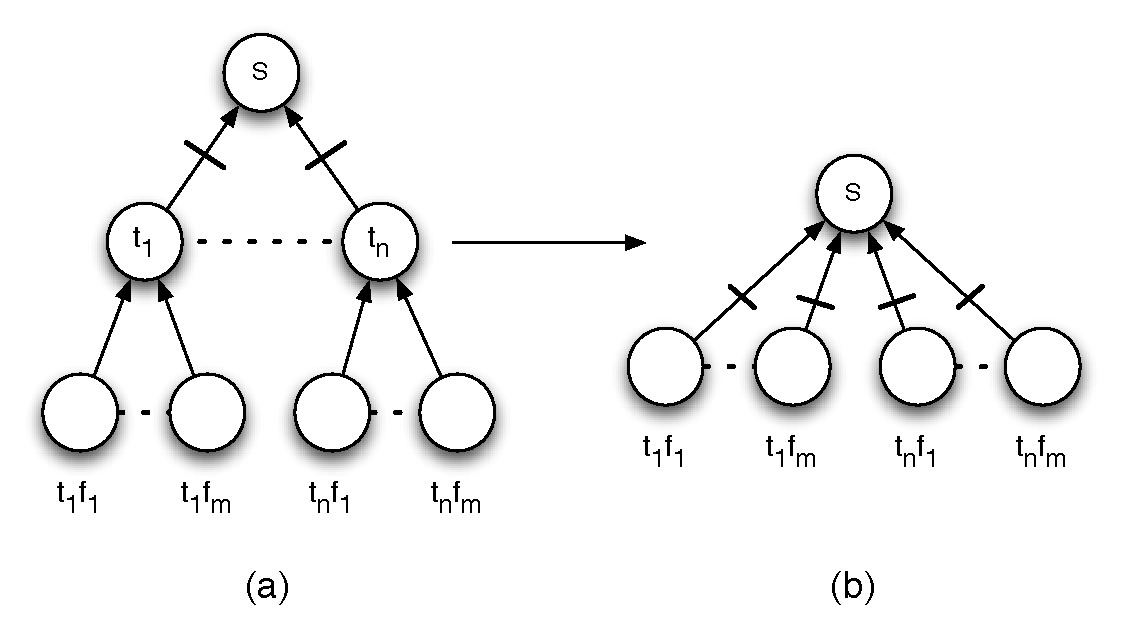
\includegraphics[scale=0.45]{imgs/modification.pdf}
\caption{Two different locations for pruning decisions. The small lines indicate where the \method{maxscore} algorithm checks to stop processing.}
\label{fig:mod}
\end{figure}
 
\section{Deriving {\large $\delta$}-Functions} \label{sec:methods}
We now describe the steps to derive a $\delta$-function. As stated above, we would like to process a document as in Fig.~\ref{fig:mod}(b), therefore we need a single function for each term-field pair that can provide the full update to the running estimate. We first describe the process algebraically, which also shows the mathematical equivalence between the original model and the $\delta$-function form. We then also describe the difference operationally via pseudo-code. This provides an intuition of how the $\delta$-functions affect scoring operationally. 
\subsection{Algebraic Description}
Using the substitution scheme defined above, we would like ${\hat \phi^{nm}} = S_{d}$, meaning after $n \times m$ substitutions, we arrive at $S_{d}$. We express $\phi$ as ${\hat \phi^{0}}$. Using these equalities, we can express the transformation of $\phi$ into $S_{d}$ via a finite telescoping series:
\begin{align}
S_{d} =& \Bigg( \cdots \left( {\hat \phi^{0}} + \left({\hat \phi^{1}} - {\hat \phi^{0}} \right) \right)  + \cdots + \left({\hat \phi^{nm}} - {\hat \phi^{(nm)-1}} \right) \cdots \Bigg) \notag \\
=&{\hat \phi^{0}} + \sum_{i=1}^{nm} \left({\hat \phi^{i}} - {\hat \phi^{i-1}} \right) = {\hat \phi^{nm}} = S_{d} \label{eq:telescoping}  \\ \notag
\end{align}
The summation form of the series provides a clean analytical representation of $S_{d}$ using the potentials. We have ${\hat \phi^{0}}$ in hand (recall all documents start with this score), therefore we need to figure out $\left({\hat \phi^{i}} - {\hat \phi^{i-1}} \right)$ for any $i > 0$. This quantity is the core of the $\delta$-function. For a given model $M$, for a given $u$ and $v$ s.t. $1 \leq u \leq n$ and $1 \leq v \leq m$, we define
\begin{equation}
\delta^{i}_{M} = \left({\hat \phi_{M}^{i}} - {\hat \phi_{M}^{i-1}} \right) = {\hat \phi_{M}^{i-1}}[\phi_{uv}/s_{uv}] - {\hat \phi_{M}^{i-1}}
\label{eq:delta-generic}
\end{equation}
which allows us to rewrite Eq.~\ref{eq:telescoping} as
\begin{equation*}
S_{d} = {\hat \phi^{0}} + \sum_{i=1}^{nm} \delta^{i}_{M}
\end{equation*}
The potential functions ${\hat \phi_{M}}$ are dependent on the model formulation, as they involve substituting in the term scoring function for that model. In general, the superscript over the $\delta$-function is implied, and we drop it to refer to the generic form. Note that the only difference between ${\hat \phi^{i}}$ and ${\hat \phi^{i-1}}$ is a single substitution. Our goal, for any given $M$, is to determine the effect of that substitution on ${\hat \phi}$. Also notice that $u$ and $v$ are not defined in terms of the previous substitutions, but just as adjustments to the current estimate ${\hat \phi^{i-1}}$. This means that we may order the $\delta$-functions in any way we like when scoring, and are not required to compose an entire term score before producing a decidable estimate. Similar to both \method{maxscore} and \method{wand}, if a document is fully scored, it is entered as a candidate for the final top $k$, and its score is accurate. Therefore this technique is both rank-safe and score-safe up to rank $k$.
\subsection{Operational Description}
Algorithm~\ref{alg:term-field-scoring} shows a standard scoring algorithm for {\daat} processing: load a document, score the terms with respect to the document, then
record the score in the result list ($R$) if applicable. Processing fields can be incorporated into the \proc{ScoreTerm} function, keeping the outer algorithm simple.  
\begin{algorithm}[t!]
\caption{A standard {\daat} scoring algorithm incorporating fields and pruning.}
\label{alg:term-field-scoring}
\begin{codebox}
\Procname{$\proc{ScoreDocuments}(Q, F, I, k, R)$}
\li $\Omega \gets -\infty$
\li \kw{foreach} document $D$ where $\exists q : q \in Q \wedge q \in D$
\li 	\Do
	$S_{D} \gets \phi$
\li	\kw{foreach} $q \in Q$
\li	\Do
		$s_{i} \gets \proc{ScoreTerm}(q, F, I)$
\li		$S_{D} \gets S_{D} + s_{i} - \phi_{i}$
\li		\If $S_{D} < \Omega$
\li		\Then
			\kw{break}
		\End		
	\End
\li	\If $S_{D} > \text{the lowest score in $R$}$
\li	\Then
		$\proc{Insert}(R, k, \langle D, S_{D} \rangle)$
	\End
\li	\If $|R| > k$
\li	\Then
		$\proc{Delete}(R, k)$
\li		$\Omega \gets$ lowest value in $R$
	\End
   \End
\li \Return \id{R}
\end{codebox}
\end{algorithm}

%\subsection{A Quick Derivation}
%As a brief example, suppose we have a new field-based retrieval model SOF, which is just a pair of nested sums over the term fields, and that we are given an admissible estimator $\phi_{ij}$. We formulate SOF, and its corresponding potential, as follows: 
%\begin{equation*}
%S_{Qd} = \sum_{i=1}^{n} w_{i} \sum_{j=1}^{m} s_{q_{i}jd} \hspace{5pt} , \hspace{5pt} \phi_{SOF} = \sum_{i=1}^{n} w_{i} \sum_{j=1}^{m} \phi_{q_{i}j}
%\end{equation*}
%The exact formulation of $s_{q_{i}jd}$ is not important. We only need access to the quantity when scoring $d$. We set up $\delta_{SOF}$ as follows:
%\begin{equation*}
%\delta_{SOF} = {\hat \phi^{i}} - {\hat \phi^{i-1}} = {\hat \phi^{i-1}}[\phi_{uv}/s_{uvd}] - {\hat \phi^{i-1}}
%\end{equation*}
%Noting that ${\hat \phi^{i-1}}[\phi_{uv}/s_{uvd}]$ reduces to simply subtracting $\phi_{uv}$ from ${\hat \phi^{i-1}}$ and then adding $s_{uvd}$ to it, we can write a simple closed form for $\delta_{SOF}$:
%\begin{align*}
%{\hat \phi^{i-1}}[\phi_{uv}/s_{uvd}] - {\hat \phi^{i-1}} =\\ 
%\left(\sum_{i=1}^{n} w_{i} \sum_{j=1}^{m} \phi_{q_{i}jd} - w_{u} \phi_{uv} + w_{u} s_{uvd} \right) -\\
%\left( \sum_{i=1}^{n} w_{i} \sum_{j=1}^{m} \phi_{q_{i}jd} \right) =\\ 
%w_{u}(s_{uvd} - \phi_{uv}) = \delta_{SOF}\\
%\end{align*}
%We now have a concrete version of $\delta_{SOF}$ we can use to score. Brief inspection of $\delta_{SOF}$ provides some intuition of its function. The quantity $(s_{uvd} - \phi_{uv})$ is negative, since $\phi_{uv} > s_{uvd}$. As we intended, each application of the $\delta$-function reduces the estimate a bit, moving it closer to $S_{Qd}$, until it has been applied for all term and field combinations. 
 
\section{Rewriting Field-Based Models} \label{sec:applied}
We now derive the $\delta$-function for the BM25F field-based ranking model. We first quickly derive an admissible UBE for term/field potentials for the model, and then proceed to develop $\delta_{BM25F}$, the $\delta$-function form for BM25F. The derivations for PRMS and PL2F can be found in Appendix~\ref{app:derivations}.

\subsection{BM25F}
%\begin{figure}
%\centering
%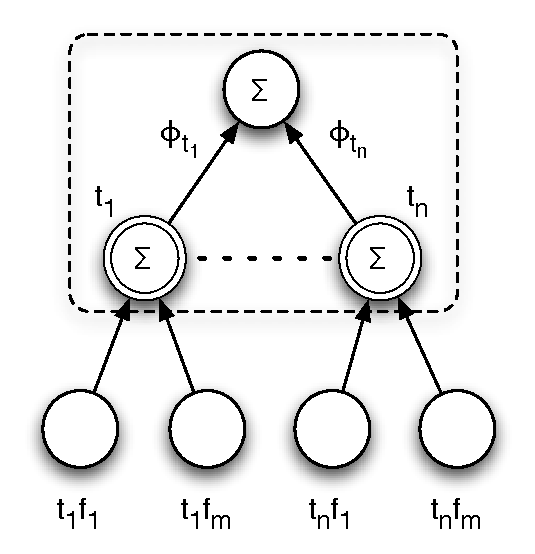
\includegraphics[scale=0.50]{imgs/bm25f-model.pdf}
%\caption{Graphical representation of BM25F.}
%\label{fig:bm25f-model}
%\end{figure}
BM25F is an extension of the BM25 retrieval model. Instead of scoring fields independently, the
term frequencies per field are first combined, then scored \cite{Robertson-cikm-2004}.
We begin by considering the set of formulae that constitute the BM25F scoring function:
\begin{align}
s_{ijd} 	&= \frac{c_{ijd}}{(1 + B_{j}(\frac{l_{jd}}{l_{j}} - 1))} \label{eq:bm25f:1}\\
s_{id}	 		&= \sum_{j=1}^{m} W_{j} s_{ijd}  \label{eq:bm25f:2}\\ 
{\bar s}_{id}		&= \frac{s_{id}}{K + s_{id}} idf_{i}  \label{eq:bm25f:4}\\
BM25F(Q,d) 			&= \sum_{t \in q \cap d} {\bar s}_{id} \label{eq:bm25f:3}\\ \notag
\end{align}
where $l_{j}$ is the average length of field $j$ across all documents, $W_{j}$ is a field-specific tuning parameter, $idf_{i}$ is the inverse document frequency of term $i$, and $l_{jd}$ is the length of field $j$ in document $d$. As before, we first find an admissible estimate for the term/field scoring function. In this model, the term/field scoring function corresponds to Eq.~\ref{eq:bm25f:1}.
\subsubsection{Finding $\phi_{ij}$ for BM25F}
We would like to create a reasonable admissable estimate we can make for any term/field pair. We use the same technique as Macdonald et al. \cite{Macdonald-tois-2011}, and view the problem as a relaxed constrained maximization problem. Let $x = c_{ijd}$, and let $y = l_{fd}$:
\begin{align*}
s_{ijd} =& \frac{c_{ijd}}{(1 + B_{j}(\frac{l_{jd}}{l_{j}} - 1))} &&= \frac{x}{(1+ B_{j}(\frac{y}{l_{j}} - 1))} \\
			=& \frac{x}{(1+ B_{j}(\frac{y}{l_{j}} - 1))} &&= \frac{x}{1 + \frac{B_{j}y}{l_j} - B_{j}} \\
			 =& \frac{x}{\frac{B_{j}y}{l_{j}} + (1-B_{j})} &&= \frac{x}{\alpha y + \beta} \\
\end{align*}
where $\alpha = B_{j}/l_{j}$ and $\beta = (1-B_{j})$. We assume both $x$ and $y$ have lower and upper bounds (e.g. $x_{max}$ is the maximum $x$ for any document). We would like to maximize $s_{ijd}$ subject to 
\begin{itemize}
\item $x \leq y$
\item $x_{min} \leq x \leq x_{max}$
\item $y_{min} \leq y \leq y_{max}$
\item $0 < x_{min} < x_{max}$
\item $0 < y_{min} < x_{max} < y_{max}$
\end{itemize}
This function monotonically increases w.r.t. $x$ and monotonically decreases w.r.t. $y$, very much like the classic functions studied before \cite{Macdonald-tois-2011}. Given our constraints, this function is maximized when $x = y$, since a constraint is that 
$x \leq y$, and in the case of $x < y$, we can find a larger value by increasing $x$ to $y$. We substitute $x$ for $y$, and take the derivative w.r.t. to $x$ to get
\begin{equation}
\frac{\partial s_{ijd}}{\partial x} = \frac{\beta}{(\alpha x + \beta)^{2}} \label{eq:gradient}
\end{equation}
which is a positive-valued function  $\forall x \geq 0$. Therefore we can follow the gradient produced in Eq.~\ref{eq:gradient} to increase the
value of $x$ until we reach it's maximum allowable value as defined by the CMP. This value is  $\argmax_{d \in D} c_{ijd}$, which we label as
${\bar x}$. 
Based on this derivation, we now have an admissible estimator for Eq.~\ref{eq:bm25f:1}. 
Therefore, for a given term and parameter $B_{f}$, we define our estimator as:
\begin{equation*}
\phi_{ij} = \frac{{\bar x}}{(1 + B_{j} \left(\frac{{\bar x}}{l_{j}} - 1 \right)}
\end{equation*}
We now proceed to derive $\delta_{BM25F}$.
\subsection{Deriving $\delta_{BM25F}$}
Similar to Eqs.~\ref{eq:bm25f:1}-\ref{eq:bm25f:3}, we define potentials for BM25F as follows:
\begin{align*}
\phi_{i} 			&= \sum_{j=1}^{m} W_{j} \phi_{ij} \\
\psi_{i} 	&= \frac{\phi_{i}}{K + \phi_{i}} idf_{i} \\
\psi 		&= \sum_{t \in q \cap d} \psi_{i} \\
\end{align*}
Modifiers described in Section~\ref{sec:term} extend to the $\psi$ quantities defined here. We start with the general version of $\delta_{BM25F}$:
\begin{equation}
\delta_{BM25F} = {\hat \phi^{i}} - {\hat \phi^{i-1}} = {\hat \phi^{i-1}}[\phi_{uv}/s_{uvd}] - {\hat \phi^{i-1}}
\label{eq:delta-bm25f1}
\end{equation}
As before, when making a single substitution, all ${\hat \psi}_{i}$ where $i \neq u$ are held constant during the substitution, and can be ignored. This leaves us with:
\begin{align}
\delta_{BM25F} = {\hat \psi}^{i-1}_{u}[\phi_{uv}/s_{uvd}] - {\hat \psi}^{i-1}_{u} \notag \\ 
=  \left( \frac{\phi_{i}[\phi_{uv}/s_{uvd}]}{K + \phi_{i}[\phi_{uv}/s_{uvd}]} idf_{u} \right) - \left( \frac{\phi_{i}}{K + \phi_{i}} idf_{i} \right) = \notag \\
 \left( \frac{\phi_{i}[\phi_{uv}/s_{uvd}]}{K + \phi_{i}[\phi_{uv}/s_{uvd}]} - \frac{\phi_{i}}{K + \phi_{i}} \right) idf_{u}  \label{eq:delta-bm25f2}
\end{align}
If we consider the semantics of ${\hat \phi}_{u}[\phi_{uv}/s_{uvd}]$ w.r.t. BM25F, we find that the substitution has a similar effect as in the PRMS case:
\begin{equation*}
{\hat \phi}_{u}[\phi_{uv}/s_{uvd}] = {\hat \phi}_{u} + W_{v}(s_{uvd} - \phi_{uv})
\end{equation*}
As both formulae use sums over the fields to generate the term values, this similarity is expected. Substituting into Eq.~\ref{eq:delta-bm25f2}, we have:
\begin{equation*}
\delta_{BM25F} = idf_{u} \left( \frac{{\hat \phi}_{u} + \xi_{uv}}{K + {\hat \phi}_{u} + \xi_{uv}} -
\frac{{\hat \phi}_{u}}{K + {\hat \phi}_{u}} \right)
\end{equation*}
where $\xi_{uv} = W_{v}(s_{uvd} - \phi_{uv})$. As in the case of $\delta_{PRMS}$, we must maintain ${\hat \phi}_{i}$ for all $q_{i} \in Q$. However using this value it is easy to compute the value of $\delta_{BM25F}$.

We perform similar derivations of the PRMS model in Section~\ref{appendix:prms} and the P2LF model in Section~\ref{appendix:pl2f}.
\section{Experimental Setup} \label{sec:experiments}
The question we want to answer is: \emph{Are \method{maxscore} and \method{wand} faster when the retrieval functions are reformulated?} Towards
answering this question, for a given collection $C$ and set of queries $Q$, we would like to compare the execution times of \method{maxscore} using the original retrieval function (\method{maxscore}$_{O}$) and \method{maxscore} using the $\delta$-function form (\method{maxscore}$_{M}$) for $Q$ executed over $C$. We run identical experiments for \method{wand$_{O}$} and \method{wand$_{M}$} as well. 
\subsubsection*{Data}
We conduct experiments over two different data sets: 1) the first 1000 queries from the Efficiency task query set from the TREC Terabyte 2006 track, over the GOV2 document collection (TB06), and 2) a download of the metadata records from the OpenLibrary (OL), along with a sample of 1000 queries from the OpenLibrary Apache logs. As we are only retrieving unigrams in these models, we stem the queries using the Porter stemmer, and we exclude stopwords from the INQUERY 418 stopword set. Table~\ref{tab:collection-stats} contains some statistics about each of the collections considered. TB06 documents have a \verb|title| field, the body content stored as the \verb|body| field, and the anchor text indexed as an additional field \verb|a|. TB06 provides a relatively standard case of web pages, with only a few fields of interest, and one of the fields significantly outweighing the others in terms of content density (i.e. the \verb|body| field is significantly bigger than the \verb|title| or \verb|anchor| fields). 

The OL records provide a contrastive dataset - there are 22 fields, none of which contain significantly more content than the rest. The records are community-built, therefore not all fields are present in all documents. The simple statistics in Table~\ref{tab:collection-stats} indicate the differing structure in OL versus TB06. The average number of tokens per field in OL is much lower than in TB06. Despite the larger number of fields, the standard deviation of the number of terms in each field is also lower. Kim et al. \cite{kim-cikm-2012} perform an in-depth analysis of this dataset\footnote{This dataset can be downloaded at: \url{http://ciir.cs.umass.edu/~hfeild/downloads.html#openLibrary2012}}.
\begin{table}
\centering
\begin{tabular}{|l|r|r|r|r|} \hline
Test Set 	& \# docs 	& terms 		& fields		&  \small{(Tokens/Field)} /  $\sigma$ \\ \hline
		& ($10^6$'s)	& ($10^6$'s)	& 	(1's)		&	($10^6$'s)	\\ \hline
TB06	& 25.2		&  22,333		& 	3		& 	5,304 / 5,870	\\ \hline
OL		& 39.4 		&  1,418		& 	22	 	& 	 64.4 / 85.2	\\ \hline
\end{tabular}
\caption{Statistics on the collections used in experiments. The last column shows the average number of tokens per field for that collection. The second value in that column is the standard deviation of the distribution of tokens per field.}
\label{tab:collection-stats}
\end{table}

\subsubsection*{Software and Hardware}
We conduct experiments using an open-source research IR system\footnote{Name anonymized for review}. The index structure is a positional index, with term-interleaved document, count, and position blocks. The document ids and positions for a given document are d-gapped, with all integers and longs compressed using vbyte encoding. Skips are implemented using a separate two-level skiplist structure. Hi-level skips record the absolute byte position every 10,000 postings, with relative skips being recorded for each block every 500 postings. If a position block contains more than 2 entries, it is prepended with the list length in bytes, to allow for skipping the structure without decompressing it.

Each run was conducted on an Intel Core2 Duo machine with 4GB RAM, with the index residing on network-mounted storage. The operating system used is Linux CentOS 5. 

\subsubsection*{Measurement}
In order to minimize the effects of network traffic, for each query we perform a warmup run of the query to load as much data into memory as possible. The primary measurement is the \textit{average latency} of a query (time to process that query). We perform 5 iterations of the warmed up query and record these numbers, forming a set of 5 samples for each query. We then take the average of the five timed runs for each query, and use that average as the representative latency of the query. All times were measured in milliseconds. 

To get a sense of the stability of these runs, in addition to the mean, we calculate the coefficient of variation of each set of query samples. The coefficient of variation is the standard deviation divided by mean, which provides a normalized measure of dispersion of a distribution. For example, a value of 0.05 indicates that the standard deviation of a distribution is only 5\% of the value of the mean. Smaller numbers indicate a higher probability that the samples are accurate measurements of the query's actual run time. These values are then aggregated for a collection, to form a distribution of coefficients. Table~\ref{tab:sample-stability} shows the quartiles for the distributions for each collection. \edit{Will fill in information here after I complete the runs and analysis.}
\begin{table}[h!]
\centering
\begin{tabular}{|l|c|c|c|c|c|} \hline
\textit{Set} 		& \textit{Min}		& \textit{1st Q} 				& \textit{Median}			& \textit{3rd Q}			& \textit{Max} 		\\ \hline
TB06	& \multicolumn{5}{c|}{ \edit{Unknown} }	\\ \hline
OL		& \multicolumn{5}{c|}{ \edit{Unknown} }	\\ \hline
\end{tabular}
\caption{Different quartiles of the distribution of coefficients of variation of queries for a particular test set. \edit{Further description pending.}}
\label{tab:sample-stability}
\end{table}

To compare two runs (say the original PRMS formulation and $\delta_{PRMS}$), we report the average drop in query latency as a ratio of the original query latency. Let $t_O$ and $t_M$ be times produced by the original (O) and modified (M) runs, respectively. We calculate the ratio improvement as $t_M / t_O$. Therefore a value of 0.9 indicates that run $M$ required only 90\% of the time taken by run $O$. A value $> 1$ indicates that run $M$ ran longer than run $O$. Therefore, a lower ratio is better. We also report the number of queries improved or worsened compared to the original formulation. We also report improvement results for the original \method{maxscore} algorithm applied to PRMS, to provide a point of comparison with a state-of-the-art approach.

We determine statistical sigificance via a two-sample permutation test as described by Efron and Tibshirani \cite{efron-bootstrap-1993}. All results are verified to be statistically significant for $p < \edit{TBD}$ unless otherwise noted. We omit retrieval effectiveness results, as the pruning algorithms are by construction safe-to-rank-k. Therefore, the top $k$ documents for a given query are receive the exact same score as the original models.

\section{Results} \label{sec:results}
\edit{ Main results presented here. Intending to include table of ratio times (similar to WWW paper), as well as a breakdown of the number of improved queries vs. worsened queries. This analysis may require a breakdown by model.}

\subsection{Analysis of Risk}
Since $\delta$-functions are new implementations of these retrieval algorithms, their computational efficiency in isolation is unknown. The results so far are very promising, but do the newly implemented functions provide any of the observed speedup, or are they actually a liability? While unlikely, it is possible to generate a particular query set such that no query processed by the system can be pruned, and every candidate must be fully scored. If the $\delta$-functions are inefficient, this could lead to significantly worse performance than changing nothing. To simulate an adversarial scenario where pruning does not occur, we force every candidate to be fully scored. 

\edit{ Results and evaluation pending. }

\section{Conclusions} \label{sec:conclusions}
We have introduced a new formulation technique for field-based retrieval models that allows systems to exploit dynamic pruning to its fullest. Our results show that direct, iterative scoring of a document allows for finer-grained level of pruning which reduces the execution time of most queries up to \edit{TBD}\%. Additionally, the results indicate that $\delta$-functions scale much better than \edit{TBD} as the number of fields increases. This property may be critical, as the structure of semi-structured documents is used more and more to improve retrieval effectiveness. 

The derivation process of $\delta$-functions is not complex. In the course of this paper we derived the $\delta$-function form for three distinct retrieval models, and realized significant gains in retrieval efficiency for each model. Although the work shown here was for field-based models, the steps for deriving a $\delta$ function for a particular model can be applied to any retrieval model. The simplicity of the process makes it attractive as a general optimization procedure for various models. Once a new retrieval model has shown its utility in retrieval effectiveness, one can simply derive its $\delta$-function to improve its overall performance, without resorting to ad-hoc solutions. 

\subsection{Future Work}
Currently potential estimations are static over the course of a query evaluation. Using ``topdocs'' to improve the retrieval efficiency has been shown to greatly cut down scoring time by providing a warmup to the scored document queue \cite{brown-topdocs, strohman-topdocs}. In addition to lowering the $R$ value for pruning algorithms, the potential of each term posting list is lowered, as the highest scoring documents are quickly scored first and do not need to be accounted for when making estimating the upper bound. We plan to investigate a similar technique that can adaptively lower the potential estimates during scoring. Doing so would trigger pruning earlier during query evaluation.

Strohman and Croft \cite{strohman-sigir-2007} describe the Refine algorithm, an approach to the term-at-a-time processing in
an in-memory index. The algorithm goes through several phases during processing, first building accumulators until scores drop too low to add an accumulator for a document that will not make the final ranked list. Eventually the accumulators are trimmed when no new documents will enter the top-$k$ set of documents (where $k$ is the number of documents requested). Finally, the remaining postings are ignored if they cannot produce a score that will cause a change in ranking in the top documents.
Since postings are skipped in a term-wise manner, the scoring organization allows that scores produced be non-safe. We believe we can use the process described here in conjunction with this algorithm. The results reported by Strohman and Croft~\cite{strohman-sigir-2007} suggest that a ``wider'' set of scorers should improve throughput. 

Recent work that builds on he \method{wand} approach is Ding and Suel's Block-Max \method{wand} (BMW) algorithm \cite{ding-sigir-2011}. The authors use a new index structure, centered on blocked posting lists, where each block is impact sorted. Using this new structure, the authors modify the \method{wand} algorithm to favor ``shallow'' (within block) reads over ``deep'' (outside current block) reads. We currently see this approach as outside the scope of this paper, as it requires considerable index reorganization to to enable BMW to operate, and a direct comparison would be confounded by the difference in index structures. We view applying $\delta$-functions in conjunction with a block-max index as future work.

Finally, we are confident that $\delta$-functions can find wider applicability in the space of retrieval models. As future work we intend to investigate the applicability of this iterative scoring method to training scenarios for learning-to-rank. If we can define a single-step update function for a given model, it could drastically reduce the computational effort needed to perform search during parameter optimization. 
%\section{Acknowledgments}
%This work was supported in part by the Center for Intelligent Information Retrieval, and in part by UMass NEAGAP fellowship. Any opinions, findings and conclusions  or recommendations expressed in this material are those of the author and do not necessarily reflect those of the sponsor.

% The following two commands are all you need in the
% initial runs of your .tex file to
% produce the bibliography for the citations in your paper.
\small
\bibliographystyle{abbrv}
\bibliography{paper}
\appendix
\section{Further Derivations} \label{app:derivations}
\subsection{PRMS} \label{appendix:prms}
The probabilistic retrieval model for semi-structured data (PRMS) by Kim and Croft \cite{kim-sigir-2010} is an extension to the language model family of retrieval algorithms which incorporates field information into the estimation of relevance. Assuming $m$ fields and $n$ query terms, the score for a document $d$ is the likelihood that $d$ would generate the query $Q$:
\begin{equation}
P(Q|d) = \prod_{i=1}^{n} \sum_{j=1}^{m} P_{\mu}(j|q_{i}) P(q_{i}|j,d) \label{eq:prms}
\end{equation}
where $P_{\mu}$ is the ``mapping probability'' that field $j$ is involved in the relevance estimation, given that $q_{i}$ appeared. The probability is estimated as follows:
\begin{equation*}
P_{\mu}(j|q_{i}) = \frac{P(q_{i}|j)P(j)}{\sum_{f_{k} \in F} P(q_{i}|f_{k})} 
\end{equation*}
We assume a uniform prior distribution for $P(j)$. In order to find $\delta_{PRMS}$, we first make sure we have, or can find, an admissible estimator for the model. $P(q_{i}|j,d)$ in Eq.~\ref{eq:prms} is a language model estimate using either Dirichlet or Jelinek-Mercer smoothing. In the terminology introduced in Section~\ref{sec:term}, $P(q_{i}|j,d)$ is $s_{ijd}$. Macdonald et al. derived $max_{tf}$ as an admissible UBE for this scoring function \cite{Macdonald-tois-2011}, and we use that estimator here. We can now define the potential of PRMS:
\begin{equation}
\phi_{PRMS} = \prod_{i=1}^{n} \sum_{j=1}^{m} P_{\mu}(j|q_{i}) \phi_{q_{i}j} \label{eq:phi-prms}
\end{equation}
Which is the value we start scoring a document from. In the following, we use $w_{ij}$ to refer to $P_{\mu}(j|q_{i})$, and  let ${\hat \phi}_{i} = \sum_{j=1}^{m} w_{ij} \phi_{ij}$ to simplify the derivation. We start with the generic form of  $\delta_{PRMS}$:
\begin{equation}
\delta_{PRMS} = {\hat \phi^{i}} - {\hat \phi^{i-1}} = {\hat \phi^{i-1}}[\phi_{uv}/s_{uvd}] - {\hat \phi^{i-1}}
\label{eq:delta-prms1}
\end{equation}
We need to concretely define ${\hat \phi^{i-1}}[\phi_{uv}/s_{uvd}]$. Given the formulation in Eq.~\ref{eq:phi-prms}, when $i \neq u$, ${\hat \phi}_{i}$ is a constant over the course of the substitution, as we are only replacing the value for term $i$ in field $j$. Therefore, the components of term $i+1$ or term $i-1$, for instance, remain unchanged. So we only need to consider the substitution's effects on ${\hat \phi}_{u}$. The composite term score is a sum of term/field estimates, therefore the substitution involves subtracting $w_{uv}\phi_{uv}$ and adding $w_{uv}s_{uvd}$:
\begin{align*}
{\hat \phi}_{u}[\phi_{uv}/s_{uvd}] = \left( \sum_{j=1}^{m} w_{uj} \phi_{uj} \right)[\phi_{uv}/s_{uvd}] \\
= \left( \sum_{j=1}^{m} w_{uj} \phi_{uj} \right) - w_{uv}\phi_{uv} + w_{uv}s_{uvd} \\
= {\hat \phi}_{u} + w_{uv}(s_{uvd} - \phi_{uv}) \\
\end{align*}
We now define $\Phi = \left(\prod_{i=1}^{n} {\hat \phi}_{i} \right)$, the product of all term estimates, and by extension $\Phi_{-u} = \left(\prod_{i=1,i \neq u}^{n} {\hat \phi}_{i} \right)$, which is the product of all term estimates, excluding ${\hat \phi}_{u}$. Note that $\Phi = {\hat \phi}_{PRMS}$ (the total estimate, possibly with substitutions). This allows us to rewrite Eq.~\ref{eq:delta-prms1} compactly:
\begin{align*}
\delta_{PRMS} &= {\hat \phi^{i}} - {\hat \phi^{i-1}} = {\hat \phi^{i-1}}[\phi_{uv}/s_{uvd}] - {\hat \phi^{i-1}}\\
&=\Phi_{-u}\left( {\hat \phi}_{u} + w_{uv}(s_{uvd} - \phi_{uv}) \right) - \Phi\\
&=\Phi_{-u}\left( {\hat \phi}_{u} + w_{uv}(s_{uvd} - \phi_{uv}) \right) - \Phi_{-u}{\hat \phi}_{u} \\
&=\Phi_{-u}\left( {\hat \phi}_{u} + w_{uv}(s_{uvd} - \phi_{uv}) - {\hat \phi}_{u} \right) \\
&=\Phi_{-u} w_{uv}\left(s_{uvd} - \phi_{uv} \right) \\
\end{align*}
The result is once again intuitive. Mulitplied out, the weighted potential $\phi_{uv}$ is removed from the total estimate, while the actual weighted contribution $s_{uvd}$ is being added. The weight is the term/field weight $w_{uv}$ multiplied by the remaining term estimates. This quantity is fairly compact, but in implementation it can be difficult to correctly maintain $\Phi_{-u}$. We can remedy this by involving ${\hat \phi}_{u}$ again:
\begin{align*}
\delta_{PRMS} = \Phi_{-u} w_{uv}\left(s_{uvd} - \phi_{uv} \right) =\\
\left( \frac{{\hat \phi}_{u}}{{\hat \phi}_{u}} \right) \Phi_{-u}w_{uv}\left(s_{uvd} - \phi_{uv} \right) = \Phi\left( \frac{w_{uv}(s_{uvd} - \phi_{uv})}{{\hat \phi}_{u}} \right)
\end{align*}

We can easily maintain cumulative scores for each term (i.e. ${\hat \phi}_{i}$), and we already have access to $\Phi$, the total estimate. In this form, $\delta_{PRMS}$ reduces to multiplying the current estimate by a small factor. As each replacement is a small negative number, the total probability slightly drops as we iterate through the different term/field pairs.

\subsection{Divergence From Randomness} \label{appendix:pl2f}
The final model we consider is the PL2F variant of the Divergence From Randomness (DFR) framework. PL2F was first introduced by Macdonald et al. at TREC 2005 \cite{macdonald-trec-2005}. The PL2F model is formulated as follows:
\begin{align}
S_{Q,d} = \sum_{q_{i} \in Q} \frac{|q_{i}|}{|{\bar q}|} \frac{1}{s_{i}+1}\Bigg( s_{i} \log\frac{s_{i}}{\lambda} +
(\lambda - s_{i}) \log e  + 0.5 \log (2\pi s_{i}) \Bigg) \label{eq:dfr}
\end{align}
where $\lambda = cf_{q_{i}}/|D|$, the collection frequency of $q_{i}$ divided by the size of the collection. $|q_{i}|$ is the frequency of $q_{i}$ in $Q$, and $|{\bar q}|$ is the maximum $|q_{i}|$ for any $q_{i} \in Q$. All log functions are in base 2 unless otherwise noted. For this model $s_{i}$ is defined as
\begin{align}
s_{i} &= \sum_{j=1}^{m} w_{j} s_{ijd} \hspace{5pt} , \text{where} \\
s_{ijd} &= c_{ijd} \log \left(1 + B_{j}\frac{l_{j}}{l_{jd}} \right) \label{eq:pl2f-scoring} \\ \notag
\end{align}
where $B_{j}$ is a field-specfic tunable parameter. We assume that $|q_{i}| = |{\bar q}| = 1$ for all terms in all queries. As before, we now derive an admissible UBE $\phi_{ij}$ before proceeding to derive $\delta_{PL2F}$. 
\subsection{Finding $\phi_{ij}$ for PL2F}
We need to generate an admissible UBE for the term/field scoring function of PL2F. Using the formulation above, that is Eq.~\ref{eq:pl2f-scoring}. We begin there:
\begin{equation*}
s_{ijd} = c_{ijd} \log \left(1 + B_{j}\frac{l_{j}}{l_{jd}} \right)
\end{equation*}
We make the same substitutions as before; let $x = c_{ijd}$, and $y = l_{j,d}$:
\begin{equation}
s_{ijd} = x \log \left(1 + \beta y^{-1} \right) \label{eq:deriv1}
\end{equation}
where $\beta = B_{j}l_{j}$. Inspection reveals that $s_{ijd}$ monotonically increases with $x$ and monotonically decreases with $y$. As before, the maximal contour is the line where $x = y$: for any case where $x < y$, we can increase the value of $x$ to $y$ to obtain a larger value. We can now substitute $x$ for $y$ to simplify Eq.~\ref{eq:deriv1} and take its derivative:
\begin{align*}
f(x) &= s_{ijd} = x \log \left(1 + \beta x^{-1} \right) \\
f^{\prime}(x) &= \frac{\partial s_{ijd}}{\partial x} = \log (1 + \beta x^{-1}) - \left( \frac{\beta x^{-1}}{(1+\beta x^{-1}) \ln 2} \right) \\
\end{align*}
We need to know the behavior of $f^{\prime}(x), \forall x > 0$. Substituting $z = \beta x^{-1}$ and taking the derivative again:
\begin{equation*}
\frac{\partial f^{\prime}}{\partial z} = \frac{\frac{z}{(1+z) \ln 2}}{((1+z) \ln 2)^{2}}
\end{equation*}
We can see that for $\frac{\partial f^{\prime}}{\partial z} > 0,  \forall z > 0$. This means that for all $x > 0$, $f^{\prime}(x)$ and therefore $f(x)$ are also positive. 
As $x \rightarrow \infty$, $f(x)$ grows unbounded. With respect to our constraints, this function maximizes at $\argmax_{d \in D} c_{ijd}$, or ${\bar x}$, as before. We now have an admissible UBE for PL2F:
\begin{equation*}
\phi_{ij} = {\bar x} \log \left(1 + B_{j}\frac{l_{j}}{{\bar x}} \right)
\end{equation*}
We can now proceed to deriving the $\delta$-function.
\subsection{Deriving $\delta_{PL2F}$}
We first determine the total potential $\phi$ for PL2F using the UBE. We define $\phi$ as:
\begin{align*}
\phi =& \sum_{i \in Q} \frac{1}{\phi_{i}+1}\Bigg( s_{i} \log\frac{\phi_{i}}{\lambda} + 
		 (\lambda - \phi_{i}) \log e  + 0.5 \log (2\pi \phi_{i}) \Bigg) \\
\phi_{i} =& \sum_{j=1}^{m} w_{j} \phi_{ij}
\end{align*}
We start with the generic formulation of $\delta_{PL2F}$:
\begin{equation}
\delta_{PL2F} = {\hat \phi^{i}} - {\hat \phi^{i-1}} = {\hat \phi^{i-1}}[\phi_{uv}/s_{uvd}] - {\hat \phi^{i-1}}
\label{eq:delta-pl2f1}
\end{equation}
The substitution takes place at field $j$ for term $i$. Given the formulation in Eq.~\ref{eq:dfr}, terms are calculated independently; we can ignore the other term quantities as they are constant over the substitution. This makes determination of ${\hat \phi^{i-1}}[\phi_{uv}/s_{uvd}]$ simple: 
\begin{equation*}
{\hat \phi^{i-1}}[\phi_{uv}/s_{uvd}] = \phi_{u} + w_{uv}(s_{uvd} - \phi_{uv})
\end{equation*}
Although the replacement over a term potential is simple, deriving a concrete form of the $\delta_{PL2F}$ is more involved. Let $\psi_{u} = {\hat \phi}_{u}[\phi_{uv}/s_{uvd}]$. We can now write the terms of concern in $\delta_{PL2F}$:
\begin{align*}
\delta_{PL2F} = {\hat \phi^{i}} - {\hat \phi^{i-1}} = {\hat \phi^{i-1}}[\phi_{uv}/s_{uvd}] - {\hat \phi^{i-1}} =\\
\frac{1}{{\hat \phi}_{u}+1}\left( {\hat \phi}_{u} \log\frac{{\hat \phi}_{u}}{\lambda} + (\lambda - {\hat \phi}_{u}) \log e  + 0.5 \log (2\pi {\hat \phi}_{u}) \right) -\\
\frac{1}{\psi_{u}+1}\left( \psi_{u} \log\frac{\psi_{u}}{\lambda} + (\lambda - \psi_{u}) \log e  + 0.5 \log (2\pi \psi_{u}) \right)
\end{align*}
In its current form the $\delta_{PL2F}$ function is not very helpful --- for every update we would have to calculate the original function twice. We can simplify this function somewhat, by establishing a common denominator between all the terms, and multiplying the two quantities out. After canceling and reducing terms, we finally end up with a less wasteful $\delta_{PL2F}$ form:
\begin{align*}
\delta_{PL2F} = \beta ({\hat \phi}_{u} - \psi_{u}) +\\
\log \psi_{u} (\psi_{u}{\hat \phi}_{u} + 0.5 {\hat \phi}_{u} + \psi_{u} + 0.5) -\\
\log \psi_{u} (\psi_{u}{\hat \phi}_{u} + 0.5 \psi_{u} + {\hat \phi}_{u} + 0.5)
\end{align*}
where $\beta = (\log \lambda + \lambda \log e + 0.5 \log 2 \pi + \log e)$.
This function is still rather bulky, however optimization of this function to use fewer operations is beyond the scope of this paper. We use this form in our implementation, and leave further optimization as future work.
\end{document}